\documentclass[letterpaper,twocolumn,10pt]{article}
\usepackage{usenix,endnotes,multirow}
\usepackage{refstyle,amsmath,chngcntr}
\usepackage{epsfig,subfigure,framed}
%\usepackage{multicol,tabularx}
\usepackage{textcomp} % for tilde

% Used for code snippets
\usepackage{listings,courier}

% Used for changing the spacing after the title, sections, and subsections.
\usepackage{titlesec,titling}

% Make text in figure captions small
\usepackage{caption3} % load caption package kernel first
\DeclareCaptionOption{parskip}[]{} % disable "parskip" caption option
\usepackage[small]{caption}

% Make sure that figure numbers are continuous through the document
\counterwithout{figure}{section}
\counterwithout{figure}{subsection}

% Settings on code listings.
\lstset{language=C,
		xleftmargin=0pt,
		xrightmargin=0pt,
		framexbottommargin=0pt,
        framextopmargin=0pt,
        framesep=0pt}

% Modify spacing before/after title, sections, and subsections.
\setlength{\droptitle}{-3em} 
\posttitle{\par\end{center}\vspace{-1.5em}}


\titlespacing\section{0pt}{5pt plus 4pt minus 2pt}{5pt plus 2pt minus 2pt}        
\titlespacing\subsection{0pt}{5pt plus 4pt minus 2pt}{5pt plus 2pt minus 2pt}   

% Compressed enumerations
\newenvironment{enumerate*}%
  {\begin{enumerate}%
    \setlength{\itemsep}{2pt}%
    \setlength{\parskip}{0pt}}%
  {\end{enumerate}}

% Compressed bibliograpgy
%\let\ORIGbibliography\bibliography
%\renewcommand{\bibliography}[1]{{\footnotesize \ORIGbibliography{#1}}}

% Add a horizontal rule above captions, and make captions closer to their figures
\DeclareCaptionFormat{ruled_caption}{#1#2#3\hrulefill}
\captionsetup[figure]{format=ruled_caption}
\let\ORIGcaption\caption
\renewcommand{\caption}[2][\compressedcaption]{%
\def\compressedcaption{#2}%
    \vspace{-12pt}%
    \ORIGcaption[#1]{#2}%
    \vspace{-12pt}}

% Decrease spacing before \paragraphs
\titlespacing{\paragraph}{%
  0pt}{%              left margin
  0.25\baselineskip}{% space before (vertical)
  1em}%               space after (horizontal)

% Prevent footnotes from spanning multiple pages
\interfootnotelinepenalty=10000

% For leaving some comments in the draft.
\newcommand{\comment}[1]{}

\begin{document}

%don't want date printed
\date{}

%make title bold and 14 pt font (Latex default is non-bold, 16 pt)
\title{\Large \bf Behave or Be Watched: Debugging with Behavioural Watchpoints}

%for single author (just remove % characters)
\author{
{\rm Peter Goodman} \hspace{1.5em} {\rm Akshay Kumar} \hspace{1.5em} {\rm Angela Demke Brown} \hspace{1.5em} {\rm Ashvin Goel}\\
University of Toronto
} % end author


\maketitle
\subsection*{Abstract}

%Finding, understanding, and fixing bugs in an operating system is challenging. Data watchpoints are a powerful tool that can help with this problem; however, hardware-based watchpoints are too scarce for many uses and software-based watchpoints lack contextual information about the watched memory.

%In this paper, we introduce \emph{behavioural watchpoints}: a new form of software-based watchpoint that simplifies the implementation of program analysis and debugging tools. Behavioural watchpoints extend on traditional watchpoints in several novel ways: they maintain context-specific information about watched memory, they watch ranges of addresses, and they invoke programmer-defined functions when watched memory is accessed. We describe three applications of these watchpoints: detecting buffer overflows, detecting read-before-write and memory freeing bugs, and enforcing fine-grained memory access policies.

%We show that behavioural watchpoints, as implemented within a kernel dynamic binary translation framework, have reasonable overheads for their intended use in analysing and debugging kernel modules.


\section{Introduction}

%A data \emph{watchpoint} is a powerful tool that reports on the usage of a particular memory location by a running program.
Despite costly effort to improve software-development methodologies, software defects in deployed codes continue to thrive causing system failure or unpredictable behaviour. Finding, understanding, and fixing software bugs is challenging and requires significant cost. Numerous tools exist to help developers identify these bugs. A data \emph{watchpoint} is one such powerful tool that reports on the usage of a particular memory location by a running program. Similar to instruction breakpoints, they correlate watched memory locations with the program points accessing these memory locations. 

There are two categories of watchpoints: i) Hardware-based approach and ii) Software-based approach. Hardware-based watchpoints are fast but scarce and requires additional hardware support. This limits their usefulness as a means of perfoming large-scale program analyses \cite{UnlimitedWatchpoints}. Software-based implementations can scale to support millions of watchpoints \cite{DynamoRIOWatchpoints}, but are limited by their view of memory as an opaque sequence of bytes. This view is at odds with program analysis tools, which require contextual information about a program's memory. Embedding such informations in existing software approach will require to maintain separate bookkeeping mechanisms which will lead to large computational and lookup overheads. This severely limits its practical and ubiquitous use and impede their adoptation by developers

In this paper, we introduce \emph{behavioural watchpoints}: a new form of software-based watchpoints which addresses the usability concern of hardware-based watchpoints and overcome the incongruency between how software implements watchpoints and how program analysis tools use them. We describes our prototype implementation of Behavioural Watchpoints using binary instrumentation and code manipulation framework and ability to watch large number of memory locations with 2x overhead. We also demonstrate how the ability to store contextual information simplify and broaden the scope of developing new debugging tools. 

 Two characteristics define behavioural watchpoints:
\begin{enumerate*}
  \item[i)] Context-specific information is embedded in each watchpoint. This information is directly available when a watched address is accessed.
  \item[ii)] The action taken when a watched address is accessed is a component of the context-specific information. This implies that different watchpoints can \emph{behave} differently.
  %\item[iii)] A single watchpoint can watch multiple addresses.
\end{enumerate*} 


%removes memory opaqueness and provide debugger useful information about the memory state thus simplifing the implementation of new program analysis and debugging tools. It also de

%Behavioural watchpoints address the usability concerns of hardware-based watchpoints and overcome the incongruency between how software implements watchpoints and how program analysis tools use watchpoints.

%Watchpoints are an integral feature of program analysis and debugging tools because they correlate watched memory locations with the program points accessing those memory locations. There are two categories of watchpoints: hardware-based and software-based. Hardware-based watchpoints are fast but scarce, which limits their usefulness as a means of perfoming large-scale program analyses \cite{UnlimitedWatchpoints}. Software-based implementations can scale to support millions of watchpoints \cite{DynamoRIOWatchpoints}, but are limited by their view of memory as an opaque sequence of bytes. This view is at odds with program analysis tools, which require contextual information about a program's memory. As a result, watchpoint-based analysis tools are harder to design and implement because they must maintain separate bookkeeping mechanisms to recover contextual information about watched memory.

%There are two categories of watchpoints: i) Hardware-based approach and ii) Software-based approach. Hardware-based watchpoints are fast but scarce, which limits their usefulness as a means of perfoming large-scale program analyses \cite{UnlimitedWatchpoints}. Software-based implementations can scale to support millions of watchpoints \cite{DynamoRIOWatchpoints}, but are limited by their view of memory as an opaque sequence of bytes. This view is at odds with program analysis tools, which require contextual information about a program's memory and severely limits its usefulness.

%In this paper, we introduce \emph{behavioural watchpoints}: a new form of software-based watchpoints that simplify the implementation of program analysis and debugging tools.  Behavioural watchpoints address the usability concerns of hardware-based watchpoints and overcome the incongruency between how software implements watchpoints and how program analysis tools use watchpoints.


%\section{Implementation}
%DBT is a useful technique for implementing dynamic program analysis and debugging tools \cite{Memcheck,DynamoRIOWatchpoints}. A dynamic binary translator is a program that rewrites the binary instructions of a ``guest" program while the guest program executes.

%Granary was the DBT framework of choice for two reasons: 
%\begin{enumerate*}
%	\item[i)] Our goal was to analyse Linux kernel modules. Granary permits fine-grained instrumentation of the instructions of a running Linux kernel module.
%	\item[ii)] Granary exposes rich type information about the Linux kernel. Granary has the ability to substitute the execution of a known function with a \emph{wrapped} version of itself. A wrapped function has the same type specification as its unwrapped counterpart and can freely modify its arguments and return value. This feature of Granary exposes type information which is used by behavioural watchpoints.
%\end{enumerate*}


%\noindent
%Behavioural watchpoints have several novel features:
%\begin{enumerate*}
%	\item[i)] {\bf Unrestricted:} A single watchpoint watches many addresses. In \Secref{buffer_overflows}, we use this feature to detect various kinds of buffer overflows.
%	\item[ii)] {\bf Extensible:} Watchpoints are easily extended by programmers. In \Secref{uninitialised_memory}, we use this feature to implement selective memory shadowing and detect reads from uninitialised memory.
%	\item[iii)] {\bf Type-specific:} When a watchpoint is added to an address, the address's type determines which set of behaviours to invoke when (displacements of) that address are dereferenced. In \Secref{access_policies}, we use this feature to detect Linux kernel rootkits by implementing fine-grained memory access policies.
%\end{enumerate*}

\section{Design}
A behavioural watchpoint is a software-based watchpoint that triggers the invocation of a function when any watched memory is accessed. Unlike most software-based watchpoints, a behavioural watchpoint watches a \emph{range} of addresses. This design supports our goal of allowing one watchpoint to monitor all memory accesses to a single object.

To achieve this design goal, we implemented watchpoints by adding an extra level of indirection to memory addresses. An unwatched address is converted into a watched address by changing its high-order bits. These high-order bits indirectly identify context-specific information about the range of memory being watched. This information, called the watchpoint's \emph{descriptor}, contains the originating watched address and a set of functions to invoke when watched memory is dereferenced. Since watchpoint information is embedded in only the high-order bits, a typical offset of a watched address is another watched address that shares the same watchpoint-specific high-order bits. A watchpoint's descriptor is indirectly located by interpreting these high-order bits as an index into a global \emph{watchpoint descriptor table} (\Figref{watchpoint_descriptor_table}). 
%Because these bits do not change, many addresses end up indirectly referring to the same watchpoint descriptor.

%\subsection{Design Implications}
Our approach has the following design implications.

%Any unwatched address can be converted into an watched address. The extra level of indirection added by watching an address allows us to efficiently locate context-specific information about the memory being watched.

%A watchpoint is added to a program by changing the high-order order bits of an address used by the program. 
%Watchpoints work on ranges instead of individual units of memory because a watchpoint is added to a program by changing 

\paragraph{A watched address must be distinguishable from an unwatched address.} All watched addresses are non-canonical addresses that trigger a hardware exception when dereferenced. We take advantage of the x86-64 architecture for implementing watched addresses. In kernel space on x86-64, canonical addresses have their 16 high-order bits set to 1. Watched addresses do not take this form. To prevent hardware exceptions, instrumentation is dynamically added to memory loads and stores. Watched addresses are detected before they are dereferenced and resolved to their unwatched counterparts (by masking the 16 high-order bits to 1). An alternative approach is to dereference a watched address and implement behavioural watchpoints in the trap handler.
	
\paragraph{Multiple watchpoints can watch the same range of memory.} Two copies of an address (e.g., two pointers to the same object) can be separately watched, so long as the high-order bits index different entries in the watchpoint descriptor table. This is useful for distinguishing between logically different objects that occupy the same memory. For example, this feature enables efficient detection of use-after-free bugs without preventing deallocated memory from being immediately reallocated for another use. This efficiency comes from our ability to have one watchpoint for the freed memory, and another watchpoint for newly allocated memory occupying the same space.
	
\paragraph{Watchpoints are viral.} If an address $A$ is watched, then every address derived from $A$ (e.g. through copying or offsetting) is also watched. This is useful for memory and taint analysis tools: a watchpoint that is added early on in the lifetime of an address (e.g., immediately before the address of some newly allocated memory is returned from an allocator) can persist and propagate until no more derived addresses exist.

\begin{figure}[t]
\begin{center}
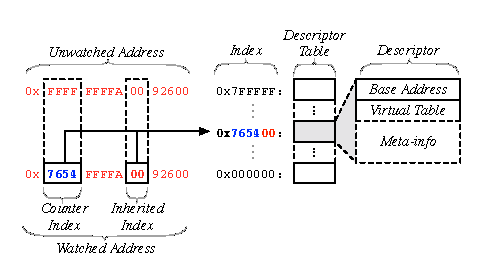
\epsfig{file=watchpoints.eps}
\end{center}
\caption{\label{fig:watchpoint_descriptor_table}A watched address (bottom left) and its corresponding unwatched address (top left) are compared. The process of resolving the watchpoint descriptor for the watched address is shown.}
\end{figure}

\paragraph{Millions of watchpoints are supported.} Our design as described uses 15 of the 16 high-order bits (called the \emph{partial index}) of a watched address for identifying a watchpoint's descriptor. 15 bits only allows 32K watchpoints. To increase the number of watchpoints, we use an additional 8 bits (bits 20-27, called the \emph{counter index}) in the address to index into the watchpoint descriptor table (\Figref{watchpoint_descriptor_table}). This counter index extends the number of possible watchpoints to 8M and is left unchanged when converting an unwatched address into a watched address. The key advantage of our watchpoint scheme is the ability to directly map watched addresses to unwatched addresses using a simple bitmask. The main drawback of the scheme is that an offset of a watched address can cause the low-order bits to overflow into the counter index. We are exploring several solutions to this problem.

%This approach has some drawbacks when an offset of a watched address causes the low-order bits to overflow into the counter index; however, we have several solutions to this problem. 

\paragraph{Watchpoint descriptors can be arbitrarily customized.} This aspect of watchpoints is possible because our design separates the allocation/management of descriptors and the addresses that they watch. Arbitrary extension of descriptors supports our goal of overcoming the incongruency between the needs of debugging an analysis tools (contextual information about watched memory), and how existing software implements watchpoints (watched memory is opaque).

%\subsection{Extensions}
%Our design includes the following extensions to watchpoints, which expand on the behavioural aspect of our watchpoint implementation.
%principally enable the \emph{behavioural} aspect of our software-based watchpoint .
%Our goal of using watchpoints to watch the memory of objects required the following 

\paragraph{Watchpoints are type-specific.} When a watchpoint is added to an address, the \emph{type} of the address determines what meta-information is included in the descriptor, as well as what functions to invoke when memory watched by the watchpoint is accessed. Two powerful applications of this extension are discussed in \Secref{type_overflow} and \Secref{access_policies}.

\paragraph{Triggered watchpoint functions are polymorphic.} The function invoked when watched memory is accessed is decided using a descriptor-specific virtual table (vtable). Each vtable provides eight functions: four read and four write functions. Each function is specific to a memory operand size (1, 2, 4, or 8 bytes). A watchpoint descriptor is initialised with either a generic or a type-specific vtable. Type-specific vtables are specific to the \emph{type} of the watched address. Behavioural watchpoints earn their name from votable because they allow watchpoints to behave differently when watched memory is accessed.

%When invoked, a vtable function operates on the watched address and its descriptor. Behavioural watchpoints earn their name from their ability to behave differently based on the meta-information stored in the descriptor and the (type-specific) vtable function invoked.

\paragraph{Watchpoints remember their originating address.} The address to which a watchpoint is first added is called its \emph{base address}, and is stored in the watchpoint descriptor. We designed watchpoints to remember their base address because it helps to ``anchor" contextual information. When a watchpoint is added, \emph{something} is known about the watched address. Later in a program's execution, an offset of the watched address might be dereferenced. Little can be said about the dereferenced address in relation to the watchpoint's originating address without knowing the originating address.

%Without the former context of why or where the watchpoint was originally added, there is little that can be said about the relation between the triggered address and 
%the watched memory except that it might be arbitrarily far away from the address to which the watchpoint was originally added.
%That is, something is known about an address when the decision to add a watchpoint to that address is made. 
%If the original address is not remembered, then it is difficult to relate a triggered watchpoint
%We designed watchpoints this way so that at any point during the lifetime of a watchpoint, 
%Watchpoints were designed this way so that contextual information is always ``anchored" to something that was once known. 

%This is consistent with our goal of using watchpoints to watch the memory of an object because we expect the base address to be the address in memory of a watched object.

%Watchpoint desc

%Because watchpoints are added to addresses, and 

%This means that 


%We can change an address into a \emph{watched address} by ensuring that a watched address is non-canonical: it cannot legally be used (on x86) without triggering a hardware exception.


%changing part of an address, not by 
%The watched range is \emph{anchored} on the address on which the watchpoint is initially added (called the base address). 

%Behavioural watchpoints are implemented by changing an address to-be-watched into a non-canonical address\footnote{In kernel space on x86, a canonical virtual address has its 16 high-order bits set to 1. Current x86 processors require that the 8 high-order bits of an address match the $9^{th}$ highest order bit.}. The translation from unwatched to watched alters the unused high-order bits of an address. 

%There are several implications of this design decision:
%\begin{enumerate}
%	\item 
%\end{enumerate}



%Behavioural watchpoints were designed with the following goals in mind:
%\begin{enumerate}
%	\item 
%\end{enumerate}


%\subsection{Architecture}

%The implementation of behavioural watchpoints distinguishes between watched addresses and their descriptors.

%A \emph{watched address} is a pointer with an index into the \emph{watchpoint descriptor table} embedded in its bits (\Figref{watchpoint_descriptor_table}). The $23$-bit index into the descriptor table is formed by concatenating bits $[20,27]$ (called the \emph{counter index}) with bits $[48,62]$ (called the \emph{partial index}). A watched address and its unwatched counterpart share the same counter index; however, the partial index of a watched address varies\footnote{This feature of watchpoints allows for a one-to-one mapping between a watched and unwatched address, and a one-to-many mapping between a watchpoint and all addresses watched by that watchpoint. The one-to-one mapping is formed by masking the high-order bits containing the partial index.}. Partial indexes are recorded in the \emph{partial index counter table}. When a watchpoint is allocated, the current value stored in the counter table for that specific counter index is incremented and returned as the watchpoint's partial index. This allocation strategy allows for at most $2^{15}$ watchpoints per counter index or megabyte of memory\footnote{x86 has byte-addressable memory. The counter index begins at bit $20$, giving each watchpoint $1$ MB = $2^{20}$ B degrees of freedom. However, if an over/underflow across the 1 MB-aligned boundary occurs then the counter index will be corrupted. We can correct one bit of corruption by requiring that the counter index and the partial index have the same sign. An alternative solution is uses a different indexing scheme. We have successfully experimented with a different indexing scheme that solves the aforementioned overflow errors, but sacrifices the one-to-one relationship between a watched and unwatched address.}.

%A \emph{watchpoint descriptor} is a data structure containing a base address, a pointer to a virtual table (vtable) of memory operations, and programmer-defined meta-information. 

\section{Implementation}
%Granary is a DBT framework that is under development. Its primary novelty is its ability to efficiently instrument arbitrary, binary Linux kernel modules without imposing overhead on the kernel. 
We implemented behavioural watchpoints using Granary: an extension of the DynamoRIO Kernel dynamic binary translation (DBT) framework \cite{DynamoRIOKernel,GranaryAtOSDI}.  Granary instruments arbitrary, binary Linux kernel modules efficiently and without imposing overhead when the core kernel is running. We plan to use Granary to analyse and debugg kernel modules, which are a frequent source of bugs and vulnerabilities in operating systems \cite{BGI,LXFI}.

Granary is unique among DBT systems because it understands and uses program type information. For example, Granary can substitute the execution of a function with a \emph{wrapped} version of itself. A wrapped function has the same type specification as its unwrapped counterpart and can freely modify its arguments and return value. Granary can wrap some module functions in this way, even if the module source code is unavailable.

While Granary provides a framework for instrumenting kernel modules, we found it was hard to write powerful instrumentation code using low-level DBT abstractions, which motivated the design of behavioural watchpoints. Next, we describe examples of watchpoint-based debugging applications that we have applied to kernel modules.

%We are developing Granary as a framework for building kernel module analysis and debugging tools. Analysing kernel modules is important because they extend the functionality and bug count of operating systems [TODO CITATION]. However, analysing module behavior is challenging. Static analysis of module source code is difficult because of the tight interaction between modules and the kernel. Some modules, however, are only distributed in a binary format, which can make static analysis intractable (on x86).



%A watchpoint is added to a previously unwatched pointer by adding an entry to the watchpoint descriptor table and embedding part of the index of the entry in the high-order bits of the pointer. The original value of the pointer is saved as the base address of the descriptor. A watchpoint is removed from a pointer by masking the high-order bits containing the partial descriptor index. This approach permits a one-to-one mapping between a watched address and its unwatched counterpart, while allowing a single descriptor to watch many addresses. Specifically, a single watchpoint can watch up to $2^{20}$ distinct addresses, and each megabyte of memory can be watched by up to $2^{16}$ distinct watchpoints.

%Watched addresses, however, do not reference valid memory. Dereferencing a watched address triggers a hardware exception. To avoid this, we use Granary to dynamically translate memory loads and stores to first check for and then resolve watched addresses to their unwatched counterparts. If a watched address is detected then a watchpoint-specific vtable function is invoked. Both the address of the watchpoint descriptor and the watched address are passed as arguments to the invoked function. Finally, the original memory instruction is emulated by one that uses the unwatched address. The choice of which vtable function to invoke depends on the size of the memory operand (1, 2, 4, or 8 bytes) and whether the operation reads or writes its operand from/to memory.

\section{Applications\label{sec:applications}}
The following sub-sections describe three applications of behavioural watchpoints and their implementations. In these sub-sections, we use the term \emph{object} to refer to a range of memory locations that are allocated together as a unit.

%to describe a value or aggregate of values stored in memory and referenced by a memory address.

\subsection{Buffer Overflows \label{sec:buffer_overflows}}
A buffer overflow occurs when a program--in an attempt to write to some object's memory--actually writes to adjacent memory cells. One method of detecting buffer overflows relies on the compiler to allocate ``poisoned" regions of memory around each object \cite{AddressSanitizer}. Small overflows (e.g., off-by-one errors) are detected by this approach because they access poisoned memory. Big overflows that ``skip" over poisoned memory and access nearby objects in memory are not detected.

Our insight is that unrelated objects will have different base addresses (i.e. the address of one object will not be derived from the base address of another), and therefore a watched object can be adjacent to a different un/watched object without conflict.

%to an unwatched one, or one with a distinct watchpoint, without conflict.
%\emph{addresses} stored in hardware registers, like high-level programming language variable names, are typically not used to simultaneously access two unrelated objects.
%Accessing poisoned memory is an error because it does not exist as a named program entity. However, 
%Our approach is similar in that memory adjacent to a watched object is considered poisoned; however, we do not rely on compiler support, nor do we allocate or mark poisoned memory as such.

We employ three overflow detection policies: heap-based, type-based, and stack-based. % All three policies depend on the same extension to the meta-information of watchpoint descriptors: a \emph{limit address}. Together, the base address (stored in the descriptor) and the limit address delineate an object's boundaries in memory \cite{BccFatPointers}.

\paragraph{Heap-based overflow detection \label{sec:heap_overflow}}
\begin{figure}
\begin{lstlisting}[language=C,basicstyle=\footnotesize\ttfamily]
FUNC_WRAPPER(__kmalloc, (size, flags), {
  void *addr = __kmalloc(size, flags);
  ADD_WATCHPOINT(addr, size);
  return addr;
})
\end{lstlisting}
\caption{\label{fig:kmalloc_wrapper}Definition of the \texttt{\_\_kmalloc} function wrapper in Granary. The above code expands into a function for wrapping the \texttt{\_\_kmalloc} kernel memory allocator. Calls to \texttt{\_\_kmalloc} are transparently substituted with calls to the generated wrapper. The wrapper invokes the original \texttt{\_\_kmalloc} function and returns a watched version of the allocated address.}
\end{figure}

The heap-based detection policy detects buffer overflow errors on all heap-allocated objects. We use Granary to wrap the kernel's memory allocator functions (e.g., \texttt{kmalloc}) and add watchpoints to the addresses returned by those allocators (\Figref{kmalloc_wrapper}). The lifetime of a watchpoint added in this way is tied to the lifetime of the memory it watches. Each watchpoint's descriptor records bounds information about the allocated memory in the form of the object's base and limit address \cite{BccFatPointers}. A buffer overflow is detected when a dereference of a watched address occurs outside of the bounds recorded by the watchpoint's descriptor (\Figref{detect_overflow}). The memory operand size-specific feature of vtable functions is helpful in catching corner cases where memory reads or writes access both an object and its adjacent memory cells, as shown in case $(3)$ of \Figref{detect_overflow}.

%intersect an object's memory and the adjacent memory cells.
%The vtable functions used by these watchpoints detects buffer overflows when a dereference of a watched address 
%memory dereferenced in a read or write falls outside of the bounds
%We use Granary to substitute invocations of the kernel's memory allocators (e.g. \texttt{kmalloc}) with wrapped versions of the allocators (\Figref{kmalloc_wrapper}). A wrapped allocator invokes the original allocator but returns a watched version of the allocated address. The lifetime of the watchpoint is 
%The watched address returned has its descriptor initialised with the base address as the allocated address and with the limit address as the base address plus the requested allocation size. All buffer overflow detecting watchpoints are initialised with the same vtable pointer.
%The vtable pointer used by all buffer overflow detecting watchpoints points to a table of memory operand size-specific functions. The operand size is necessary to detect dereferences of memory that overlap both the object and its adjacent memory, as illustrated in case \emph{(3)} of . The vtable function corresponding to the memory operand size is invoked when a watched address is dereferenced. Each vtable function is programmed to check the watched address against the base and limit addresses stored in watchpoint's descriptor (\Figref{detect_overflow}). If a buffer underflow or overflow is detected then the vtable function notifies the run-time system.

\begin{figure}
\abovedisplayskip=0pt
\belowdisplayskip=0pt
\begin{center}
	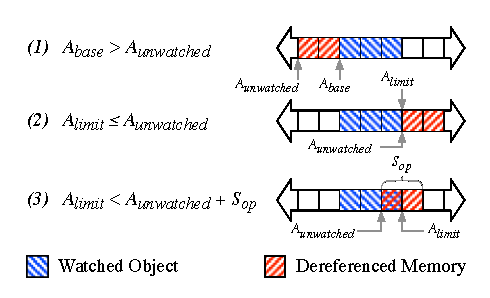
\epsfig{file=overflow.eps}
\end{center}
\iffalse
	\abovedisplayskip=0pt
	\belowdisplayskip=0pt
	\begin{align*}
		A_{base}  & > {A_{unwatched}} \tag{Underflow} \\
		A_{limit} & \leq {A_{unwatched}} \tag{Overflow} \\
		A_{limit} & < {A_{unwatched}} + S_{op} \tag{Overlap}
	\end{align*}
\fi
\caption{\label{fig:detect_overflow}Three common buffer overflow cases are illustrated above: 1) underflow 2) overflow, and 3) overlap. Beside each illustration is the policy that detects the specific bug. When a watched address ($A_{watched}$) is dereferenced, a vtable function that is specific to the memory operand size ($S_{op}$) is invoked. This function detects a buffer overflow if the intended referenced memory address ($A_{unwatched}$) does not fall within the boundaries delineated by the base and the limit addresses ($A_{base}$ and $A_{limit}$, respectively).}
\end{figure}

\paragraph{Type-based overflow detection\label{sec:type_overflow}}
Type-based overflow detection is applied when the type of an object is known. It is distinguished from heap-based overflow detection in that it can apply both to heap and non-heap memory, and it can be used to inform the run-time system about more accurate bounds information. In all other respects, the type-based overflow detection policy detects bugs in the same way as the heap-based policy (as might be encoded within the fields of a vector-like data structure).

% If the type of an object is known then it can reveal semantic relationships which can enable further type- or heap-based overflow detection. For example, the fields within a structure might encode memory bounds information (as would be the case for a vector-like data structure)

%The type-based detection policy is applied when the type of a pointer is known (i.e. not \texttt{void*}). The simplest use case of type information is to infer the limit address of a typed pointer. A more complex use case arises when the fields within a structure encode memory bounds information. In both cases, the vtable functions for typed and untyped memory operate in the same way.

The type of an addressable object becomes known to Granary in the context of a wrapped function. The run-time system performs a type-specific initialisation of a watchpoint's descriptor when a watchpoint is added to a pointer/address with a known type. Type-specific descriptor initialisation is a powerful feature because it allows for new watchpoints to be lazily added (thus propagating our detecting capabilities) to newly discovered objects referenced \emph{within} an object of a known type. We automatically propagate type-based watchpoints using type specifications generated from parsing \texttt{C} header files. Some manual post-processing is required if one is to inform the system of semantic relationships between function arguments or structure fields.

%use a type-specific vtable instead of a generic vtable when watching a typed pointer. Granary includes a database of 


%Granary recursively follows argument and return value pointers based on object type specifications. These specifications tell Granary how to follow pointers and what--if any--pointers should be converted to watchpoints. To reduce programmer effort, Granary automatically generates type specifications and wrapper functions for any set of known types and functions. Some manual post-processing is required if the analysis/debugging application needs to understand semantic relationships between function arguments or structure fields. \comment{Automating this process was an important goal of Granary because of Granary wraps all (approx. 6,000) exported kernel functions.}

\paragraph{Stack-based overflow detection}
%We detect overflows on stack allocated objects when memory outside of the bounds of the activation/call frame in which the object is allocated is accessed. This policy is distinguished from the heap- and type-based policies in that the watchpoint descriptor is managed separately from the watched memory, and the lifetime of the descriptor extends beyond the lifetime of the watched memory.

To detect stack overflows, we view the memory occupied by the activation frame of an invoked function as a dynamically-sized buffer. Like our other buffer overflow policies, we use a watchpoint to detect accesses to memory outside of this buffer. Unlike our other policies, we only \emph{associate} a descriptor with this buffer, and rely on a different mechanism to \emph{add} the watchpoint to stack addresses.

%, and manage what addresses are watched with this descriptor using a separate mechanism.

We separate adding watchpoints from allocating descriptors for stack overflow detection. In particular, we associate a descriptor with the buffer represented by the activation frame of a called function. This descriptor tracks the bounds of the frame over the lifetime of the function call. We update the recorded bounds of the frame (in the descriptor) when the frame grows or shrinks. When a function returns, the descriptor's bounds shrink to zero, but the descriptor remains allocated.

%We add an activation frame's watchpoint to a stack address under two circumstances. 

Separately managing descriptors allows us to optimize for the two most common sources of stack overflows and ignore instructions that are likely to be safe. First, if we see an instruction that copies the stack or frame pointers, then we assume that the copied address can escape the function. A stack address escaping a function is a potential stack-overflow risk. Adding the frame's watchpoint to this address \emph{taints} the copied address. Future copies or displacements of the watched address implicitly propagate its taintedness because offsets of a watched address reference the same descriptor. A dereference of an escaped pointer--even one happening after the function has returned--is detected as an overflow because the watchpoint descriptor remains live. Second, if we see an indexed dereference of the stack or frame pointers that uses a dynamically bound index, then we assume that the effective memory address accessed is a potential stack-overflow risk. We translate the dereferencing instruction to add the frame's watchpoint to the effective address before the address is dereferenced.

%and addresses that we want to have watched by 
%Under this lens, we associate a watchpoint descriptor with each function call that tracks the bounds of each activation frame. 
%allocating one watchpoint descriptor for each function call. This descriptor exists to track the bounds of the activation frame over the lifetime of the function call. The run-time system dynamically adds instructions to the instrumented program that change the recorded bounds when the size of the activation frame grows or shrinks. When a function returns, the descriptor's bounds shrink to zero.

%Instrumentation is dynamically added to the program that increase/decrease the recorded size of the activation frame in the descriptor when the 
%The descriptor tracks the size of the activation frame

%Unlike the heap- and type-based overflow policies, there are numerous optimisations 
%Stack-based overflow detection is distinguished from the heap- and type-based policies in that numerous optimisations are possible, and that 
%in an access to memory outside of the object's activation frame.
%The aforementioned approaches to overflow detection 
%Stack-based overflow detection is distinguished from the heap- and type-based overflow detection policies insofar as it uses 

%Detecting stack overflows is important because they are commonly used in remote code execution and privilege-escalation attacks against operating systems \cite{SecureProgramExecFlowTracking}.

% more support from Granary's run-time system. At a high level, each activation frame is assigned a dedicated watchpoint when a function is called. The effect of an instruction that grows or shrinks an activation frame's size is reflected by a similar change to the base address\footnote{The run-time call stack on x86 grows into lower memory.\comment{ Modifying the base address instead of the limit address allows us to maintain one set of vtable functions for all three buffer overflow detection policies.}} of the frame's watchpoint descriptor. When a function returns, the descriptor of its activation frame is cleared, but remains allocated\footnote{Reclaiming/reusing allocated but unlikey-to-be-used watchpoints is challenging. One overflow-specific approach is to ensure that the next use of the watchpoint is for a buffer whose bounds do not intersect with the current use's bounds. Another approach is to use some number of context switches as a grace period in which the watchpoint cannot be reused, but after which it can be reused. We leave this as future work.} lest the address of a local variable escape the function\footnote{If the address of a stack-allocated object escapes its function activation frame, then that pointer is said to be \emph{dangling}. Dereferences of dangling pointers can cause stack overflow errors. In the kernel, data stored in unallocated stack memory (e.g. through a dangling pointer) is at risk of being clobbered by interrupt stack frames and by function activation frames.}.  

%We assume that a memory instruction operating on a constant displacement of the stack or frame pointer registers is well-behaved. However, if the stack or frame pointer registers participate in a memory instruction and the displacement from the register is dynamically-bound then that instruction is suspect. An instruction that copies the address in the stack or frame pointer registers is also suspect because the copied address might escape the current function or participate in a local stack overflow. All suspect instructions are translated to transparently add the frame's dedicated watchpoint to the dereferenced or copied address.

%This scheme segments the runtime stack into contiguous but non-overlapping regions of watched memory. A straightforward extension excludes saved return addresses and link pointers from the known bounds of activation frames, thus detecting return-oriented buffer overflow attacks.

\subsection{Selective Memory Shadowing\label{sec:uninitialised_memory}}

In this section, we show how to use behavioural watchpoints to shadow memory. Previous work has focused on full memory shadowing \cite{Memcheck}, while watchpoints enable \emph{selective} shadowing of watched objects. We describe how the initialisation state of each byte of watched memory is tracked using shadow memory, and how to detect bugs related to the usage of heap-allocated memory.

We use Granary to wrap kernel memory allocators and deallocators (e.g., \texttt{kmalloc}, \texttt{kfree}). Wrapped allocators add watchpoints to the addresses returned by the kernel's allocators, and wrapped deallocators remove watchpoints before invoking the kernel's deallocators. Selective shadow memory is maintained as a watchpoint descriptor-specific, variable-sized bitset\footnote{As an optimisation, shadow memory for small objects is embedded in the watchpoint descriptor.}. Each byte of allocated memory corresponds to one bit of descriptor-specific shadow memory. The bits in shadow memory are initialised to zero. Individual bits are flipped to one by write-specific vtable functions when there is a write to the bytes of memory shadowed by those bits. 

%When a wrapped allocator is invoked, a watchpoint is added to the addresses returned by those allocators
 

% in shadow memory are initialised to zero.
%Watchpoints are added to all heap-allocated objects 
%the meta-information within each watchpoint descriptor.
%By tracking the initialisation state, we detect


%We apply the above shadow memory scheme to detect uses of uninitialised memory for heap-allocated objects. As in \Secref{heap_overflow}, we interpose on the kernel's memory allocators and add watchpoints to the addresses returned by those allocators. When memory is allocated, the watchpoint descriptor is initialised with the number of allocated bytes (available as an argument to the allocator) and with its own shadow memory. 

%detect uses of uninitialised memory.  Detecting such uses is important because a program using uninitialised memory can exhibit unintended, non-deterministic behaviour.

%We define uninitialised memory as either allocated memory to which no value has been written, or de-allocated memory. We selectively track the initialisation state of each byte of watched memory using \emph{shadow memory} \cite{Memcheck}. Our implementation represents shadow memory as a bitset, where the state of each bit tracks the initialisation state of a byte of watched memory. Watchpoint descriptors are augmented to include the size (in bytes) of a watched object and a pointer to the memory shadowing the object\footnote{As an optimisation, shadow memory for small objects can be embedded in the watchpoint descriptor.}.



\paragraph{Read-before-write bugs}
Read-specific vtable functions detect read-before-write bugs by checking if the shadow bit corresponding to one of the read bytes is zero. However, this method of detection can report false positives: it is common for larger-than-needed reads to be performed and for compiler-added structure padding to be read (but never written). A relaxed version of our read-before-write memory checking policy requires that at least one shadow bit is set for every read operation.

\paragraph{Memory freeing bugs}
We detect freeing of non-heap memory when the argument to a kernel memory deallocator is not a watched address. We detect an invalid-free when the unwatched address (computed through masking) of a watched address being deallocated is different than the watchpoint descriptor's base address. We detect use-after-free bugs by marking the descriptor of a watched address being deallocated as dead. The lifetime of a dead descriptor extends beyond that of the object so that a later use of any watched address with that descriptor will report a use-after-free bug. We detect double-free bugs when the descriptor of a watched address being deallocated is already marked as dead.

%We use Granary to wrap the kernel's deallocation functions (e.g. \texttt{kfree}). Because all allocators are wrapped and add watchpoints, freeing of non-heap memory is easily detected when  

%We detect freeing of non-heap memory 

%If the argument to a wrapped deallocator function is a watched address then the shadow memory for the . 

%Finally, the original deallocator is invoked with the unwatched address as an argument. Reads and writes to a watched address of a deallocated object fail to pass bounds checks because the object size is zero.

%Two positive side-effects of our approach is that it detects double-free bugs and freeing of non-heap memory bugs. A double-free is detected when a watched address for an already deallocated object is passed as an argument to a deallocator. An attempt to free non-heap memory is detected when an unwatched address is passed as an argument to a deallocator.

\subsection{Field-grained Access Policies\label{sec:access_policies}}

\begin{figure}[t]
\begin{lstlisting}[language=C,basicstyle=\footnotesize\ttfamily]
// Invariant: rtc_fops->ioctl == &rtc_ioctl
WATCH_WRITE(struct file_operations, ioctl, {
  if(&rtc_fops  == base_address
  && &rtc_ioctl != ioctl) {
    // potential attack: prevent an anti-
    // virus scan from being scheduled!
  }
})
\end{lstlisting}
\caption{\label{fig:field_invariant_check}This code example shows how to check invariant 1(h) from \cite{GibraltarKernelInvariants} using Granary's field-accessor API. The invariant checked prevents a (potential) kernel rootkit from installing its own \texttt{ioctl} handler into the Real-Time Clock. Anti-virus programs depend on this built-in \texttt{ioctl} handler to periodically schedule virus scans. Replacing this handler can prevent such scans from being scheduled, thus allowing the rootkit to go undetected.}
\end{figure}

In this section, we briefly describe using watchpoints at the granularity of object fields. Using a field-accessor API, we detect Linux kernel rootkits, which is challenging because rootkits actively try to hide their existence. However, rootkits often leave hints of their existence in the form of violated data structure invariants \cite{GibraltarKernelInvariants,OSck}.

\Figref{field_invariant_check} shows an example use of the field-accessor API that checks an invariant on the \texttt{ioctl} field of any watched object whose type is \texttt{struct file\_operations}. A rootkit violating this invariant can prevent an anti-virus program from scheduling periodic scans---scans which might otherwise detect the presence of a rootkit. However, a violation of this invariant is immediately detected by our run-time system because the field-accessor API enables active rather than passive checking of invariants.

The field-accessor API connects to type-specific watchpoint vtables through automatically generated code. Generating this code involves parsing \texttt{C} structure type layout information from the \texttt{C} header files of the Linux kernel.

\section{Evaluation}
%\begin{figure*}[t]
%\begin{multicols}{2}
%{\footnotesize
%\begin{tabularx}{\columnwidth}{l|l|c}
%Benchmark & Benchmark Description & Result \\
%\hline
%Microbenchmark & Tight loop of watched dereferences & 20x \\
%\texttt{rcutorture} & Slowdown of reader threads & 7.5x \\
%IOZone & Slowdown of reader threads & 7.5x \\
%Netperf & Slowdown of reader threads & 7.5x \\
%\end{tabularx}}
%\noindent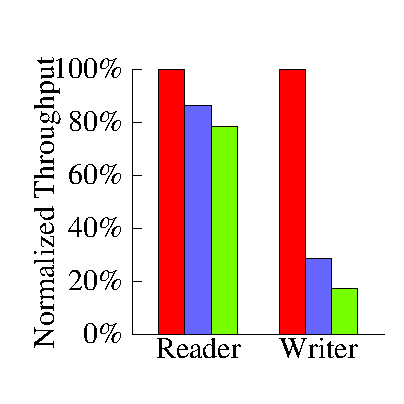
\epsfig{file=iozone.eps,height=100pt}
%\end{multicols}
%\end{figure*}

We evaluated the performance of behavioural watchpoints using a microbenchmark, Netperf, and IOzone. Our tests ran on a desktop equipped with an Intel\textregistered\ Core\texttrademark\ i7-860 2.80 GHz CPU, 8GB memory, and an Intel 82578DM Gigabit Ethernet card. Watchpoint instrumentation was enabled for every memory load and store, and buffer overflow detecting watchpoints were added to all memory returned from kernel heap allocators.

%We compare native execution, passive execution, and active execution to evaluate the performance of our watchpoint implementation. Passive and active execution both run the Granary DBT framework; however, passive execution only performs basic translation of module code, while active execution translates and adds watchpoint-specific instrumentation to module code. Our choice of network and filesystem modules depend on the fact that they are

\paragraph{Microbenchmark} The microbenchmark performed a tight-loop of memory operations and exhibits the worst-case performance overhead of watchpoints (about 20{\footnotesize$\times$}). This is expected because our instrumentation adds roughly 13 instructions to each memory load and store. 

%\paragraph{\texttt{rcutorture}} We tested the \texttt{rcutorture} kernel module. It exhibited interesting behaviour: all threads experienced a minimum of 6{\footnotesize$\times$} overhead; however, readers were abnormally penalized and tended to see more stale data. We think this is because each writer synchronized with fewer readers.

\paragraph*{Netperf} We tested network throughput and latency using the \texttt{e1000e} network device driver module. CPU utilization increased by {\texttildelow}6\%, UDP throughput decreased by at most 50\%, TCP throughput was unaffected, and both the TCP and UDP request-response latency increased by no more than 50\%. 

\paragraph*{IOzone} We tested the throughput of disk read and write operations with the \texttt{ext3} file system module, a file size of 512Kb written in 4Kb records, and with a single reader/writer thread in each case. The throughput for reads and writes decreased by  {\texttildelow}20\% and {\texttildelow}80\%, respectively.

%the throughput of file reads by a single reader thread decreases by , and the throughput of file writes by a single writer thread decreases by {\texttildelow}80\%.
%Our testing environment includes running our system with active (actively looking for watchpoint) and passive (null instrumentation) mode.
%On the microbenchmark, passive instrumentation has a 4\% overhead and active instrumentation has a 20x overhead. For the \texttt{rcutorture} module, 
%the overhead of passive instrumentation is 4\% and the overhead of active instrumentation is 20x
%under a worst-case scenario with a microbenc
%Our evaluation of the performance of behavioural watchpoints 

\section{Related Work}
%Watchpoints are an important debugging facility that help developers track accesses to memory. Most state-of-the-art processors provide some support for hardware watchpoints, but such watchpoints are usually scarce or require specialised hardware support \cite{Mondrix,UnlimitedWatchpoints}. 

\paragraph{Hardware-based}
Greathouse \emph{et al.}~\cite{UnlimitedWatchpoints} propose a hardware solution that efficiently supports an unlimited number of watchpoints. Witchel and Asanovic \cite{Mondrix} describes the implementation of memory protection domains for the Linux kernel. Protection domains are implemented using specialised hardware and enable fine- and coarse-grained memory protection using a mechanism similar to hardware watchpoints. Unlike our approach, both \cite{Mondrix} and \cite{UnlimitedWatchpoints} depend on specialised hardware and require that applications using this hardware  separately maintain context-specific information. Suh \emph{et al.} \cite{SecureProgramExecFlowTracking} proposes a method of secure program execution by tracking dynamic information flow. Memory tagging at the hardware level allows their system to track tainted data as it propagates through a running program. Behavioural watchpoints are similar insofar as a watched address is tagged, and this tag propagates through a program.


%makes the case for supporting an unlimited number of watchpoints. A hardware solution is proposed and multiple applications are described. Unlike our approach, the cited approach depends on specialised hardware and requires that applications using these watchpoints maintain their own context-specific information.

%In , 

\paragraph{Software-based}
Zhao \emph{et al.} \cite{DynamoRIOWatchpoints} describe a method of implementing an efficient and scalable DBT-based watchpoint system. His method uses page protection and indirection through a hash table to track watched memory. This approach does not support watching ranges of memory, nor does it support context-specific information. Lueck \emph{et al.} \cite{PinADX} introduce semantic watchpoints as part of the PinADX system, an extension of the PIN DBT framework. PinADX enables interactive debugging by triggering debugger breakpoints when semantic conditions are met. While similar in spirit to behavioural watchpoints, semantic watchpoints do not maintain context-specific, per-watchpoint state. 

%In this respect, a semantic watchpoint is similar to a behavioural watchpoint whose vtable functions trap when a semantic condition is met.
% using DynamoRIO, a popular user-space DBT framework. The method described is very efficient, but unlike behavioural watchpoints, views memory as an opaque sequence of bytes. 
%There have been several proposals on implementing watchpoints in software. 
%Zhao introduced a method for supporting millions of software-based watchpoints using DynamoRIO, a popular user-space DBT framework \cite{DynamoRIOWatchpoints}. Their method is very efficient and does not require inspecting all memory. 
%Our approach differs from theirs in that we e
%Our approach differs from them in the sense that our watchpoint contains the contextual information which can be used for debugging. 
%In , 
% can add a data breakpoint at an address and any access of the gets checked. Unlike this our approach of behavioral watchpoint watches the range of addresses and a watchpoint monitors the access of an object.  Our approach of watchpoint is also viral and any address derived from the watched addresses will also get watched. Our watchpoint implementation bears a resemblance with {cite dynamic information flow} however we don�t require hardware support to efficiently store the tag else it gets embedded with the address itself.


\section{Conclusions and Future Work}
%We created behavioural watchpoints with the goal of simplifying the implementation of program analysis and debugging tools. We implemented behavioural watchpoints in software because hardware approaches to watchpoints do not meet the needs of program analysis tools. We identified an incongruency between how existing software implements watchpoints and how program analysis tools use watchpoints. Finally, we overcame this incongruency by developing a new form of watchpoint that maintains its own context-specific information---information that is required for large-scale program analysis. We demonstrated the usability of behavioural watchpoints by describing the implementation of three memory error detection and protection policies.

We created behavioural watchpoints with the goal of simplifying the implementation of program analysis and debugging tools. Behavioural watchpoints are a new form of software watchpoint, which address both the scalability limits of hardware watchpoints and the lack of contextual information with traditional software watchpoints.  The key innovation is to maintain context-specific information about the memory being watched---information that is required for large-scale program analysis---with the watchpoint itself.  Thus, behavioural watchpoints resolve the incongruency between how existing software implements watchpoints and how program analysis tools use watchpoints. We demonstrated the usability of behavioural watchpoints by describing the implementation of three memory error detection and protection policies.  Although our evaluation is limited at this stage, the overheads of behavioural watchpoints, as implemented in Granary, are quite reasonable for the target use of debugging kernel modules.

As future work, we will investigate the applicability of behavioural watchpoints as a means of isolating and enforcing control-flow integrity policies on Linux kernel modules.


%Behavioural watchpoints make it easier to implement program analysis and 

%overcome the incongruency


%We have established that behavioural watchpoints are useful for implementing memory error detection and protection policies. In summary, we conclude.

% The bibliography should be embedded for final submission.
\bibliographystyle{acm}
\bibliography{library}
\end{document}


